%# -*- coding: utf-8-unix -*-
%%==================================================
%% chapter03.tex for SJTU Master Thesis
%% software requirement specification
%%==================================================
%\bibliographystyle{sjtu2}%[此处用于每章都生产参考文献]

\chapter{相似轨迹查询系统设计}
\label{chap:system requirement specification}

\section{本章序言}
\label{sec:introduction}
随着相似轨迹查询这以在科研领域和工业应用中的不断发展,开发相似轨迹查询系统为用户在搜索相似轨迹中提供更方便更可视化的结果。为了明确关于相似轨迹查询系统的设计需求、应用领域与系统功能,在本章节中,本文首先对相似轨迹查询系统的设计与实现作细节说明和具体描述。我们对本章节的目的以及之后说明中会涉及到的名词概念进行解释,以便于之后章节的拓展。该系统是主要以Python进行后端数据处理,系统运行于以Python为基础的Flask Web内部依赖Werkzeurg的工作集服务器。用户只需要通过进行简单操作便可以实现个性化的相似轨迹查询操作,并了解本系统软件的基本工作原理。


\subsection{系统应用范围}
\label{subsec:scope}
相似轨迹查询系统是一个基于\emph{GPS}轨迹数据的服务器端应用系统。根据轨迹用户提供的输入轨迹或一组基于GPS数据的轨迹点集,系统帮助用户在地理语义上查询出与输入最相似的k条结果轨迹。系统可以免费从Github上下载并运行在可以运行Python程序的平台上。

本系统在应用中,需要连接互联网以调用基于Javascript的地图服务接口,实现地图显示和轨迹显示等等基础功能。所有系统所需要的轨迹数据以文件系统存储于服务器端。在系统运行过程中,用户可以通过浏览器登录页面进行系统访问,结合用户自身查询需求系统得出不同的查询结果。本系统也支持展示出所有地图上具体位置信息和查询具体地理位置的功能。


\subsection{系统名词定义}
\label{subsec:definitions}
表\ref{tab-system definitions}所示。
\begin{table}[!htpb]
  	\centering
		\begin{tabular}{ |p{3cm}||p{9cm}|  }
		\hline
		符号标记 & 符号注释 \\
		\hline
		用户 & 使用相似轨迹查询系统进行轨迹查询人员 \\
		\hline
		管理员 & 相似轨迹查询系统管理员,负责运行权限和控制系统 \\
		\hline
		轨迹数据 & 移动物体上空间上按时间顺序的移动数据记录 \\
		\hline
		GPS & 全球定位系统 \\
		\hline
		DESC & 描述 \\
		\hline
		DEP & 依赖 \\
		\hline
		\end{tabular}
	\bicaption[tab-system definitions]{相似轨迹查询系统涉及名词定义}{相似轨迹查询系统涉及名词定义}{Table}{A list of definitions and explanations in the system of searching similar trajectories}
\end{table}

\section{大体描述}
\label{sec:overall description}
本文设计的相似轨迹查询系统运行运行于基于Python语言的Flask Web框架,运行过程中需要连接互联网以使用地图接口,系统内部数据为上海私家车数据。系统针对的用户为一般用户和登录用户。一般用户可以目的轨迹点集进行相似轨迹查询,实现路径规划等具体应用,用户在运用过程中需要在地图上点击位置以实现轨迹点击输入;登录用户在一般用户具有功能基础上,用户的历史轨迹在轨迹数据库中有存储,可以实现以一条轨迹为输入的相似轨迹查询,实现拼车或轨迹推荐等具体应用。本系统目前已有依赖于Flask框架和地图接口提供。

\subsection{系统设计框架}
\label{subsec:product perspective}
相似轨迹查询系统主要由前后端两部分组成。后端部分主要以轨迹预处理、相似轨迹查询和查询请求分析处理为主;前端以部分地图轨迹可视化、查询结果输出、地理位置搜索等部分组成。

针对相似轨迹查询系统的后端处理流程思路主要为,在后台运行服务器代码,接收来自浏览器前端的请求。将请求分析与提前预先设定的资源定位符函数结合,对于数据类型选择是否进行轨迹数据预处理。针对同一的输入轨迹数据点集,进行相似轨迹数据查询功能服务。然后将结果作为请求返回返回给用户。实现一次相似轨迹查询请求过程。与此同时,系统前端主要以实现数据可视化为主,以一个窗口形式将地图数据显示。对于用户感兴趣的地理位置坐标点和历史轨迹数据,可以通过点击地图或历史轨迹数据项目将数据在地图窗口上得以可视化展示。

\begin{figure}[!htp]
  \centering
  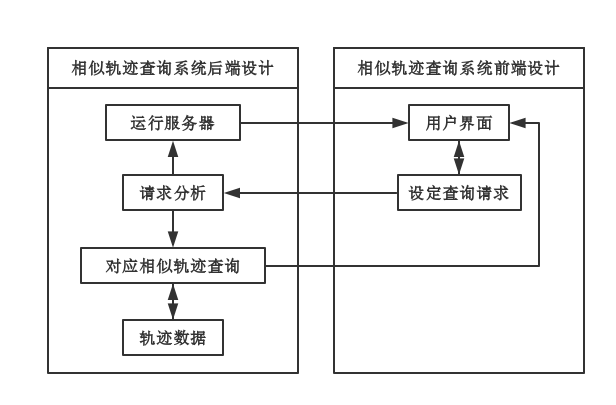
\includegraphics[width=0.8\textwidth]{specification/system-architecture.png}
  \bicaption[fig:system-architecture]{相似轨迹查询系统设计框架}{相似轨迹查询系统设计框架}{Fig}{System design architecture}
\end{figure}

\subsection{系统功能描述}
\label{subsec:product functions}
在相似轨迹查询系统中,一般用户和登录用户都可以使用相似轨迹查询功能。查询结果与用户定义的输入轨迹数据类型(为轨迹点集或一条历史轨迹)、查询的日期、相似轨迹数目阈值和查询是否有序性有关。

相似轨迹查询的主要是通过在地图上以不同颜色和不同粗细的折线端进行表示。在查询结果中,根据与查询输入相似度的相关性,越相似的查询结果轨迹将以越显著的参数表示出来,用户可以一目了然在地图上得出最符合查询的结果的一条或多条轨迹。

\subsection{系统限制描述}

\subsection{用户类与特点}
\label{subsec:user characteristics}

\section{系统具体需求分析}
\label{sec:overall description}


\subsection{系统需求说明目的}
\label{subsec:propose}
在完成对相关工作的研究和系统市场的前景分析后,本文提出相似轨迹查询系统设计需求说明。相似轨迹查询查询系统设计需求说明的目的在于对于本系统进行具体描述,明确索要开发的系统应该具备的功能与界面,为系统分析及移植开发提供清晰的基础需求描述,并以此为基础进一步满足后续设计与开发。本文所设计开发的相似轨迹查询系统目标是为用户提供高效、准确的查询服务平台。系统针对目前轨迹信息管理的实际情景,较为全面地满足用户的查询需求,初步实现系统所制定的设计初衷。需求说明从字面上作为软件系统发展的指导和完备部分,解释说明了系统中的限制条件、应用交互接口以及具体功能。


\subsection{用户界面需求}
\label{subsec:external interface Requirements}

\subsection{用户功能需求}
\label{subsec:user class functional requirements}


